\section{Theory}

Compoton scattering is a physical event that validated the dual nature of light, which had been previously established in photoelectric effect.This phenomenon is essential in medical imaging, astrophysics, and material science, aiding in X-ray diagnostics, cosmic radiation studies, and non-destructive
testing. The phenomenon involves the scattering of a photon from a metal object. The photon collides with an electron within the target, losing part of its energy due to the collision principle of conservation of energy and momentum (Fig. \ref{th:1}). Similarly, the photon changes its propagation path, resulting in varying intensities of detection at different angles, but the electron is expelled from its starting state and, following energy absorption, excites to a higher energy level.

\begin{figure}
    \centering
    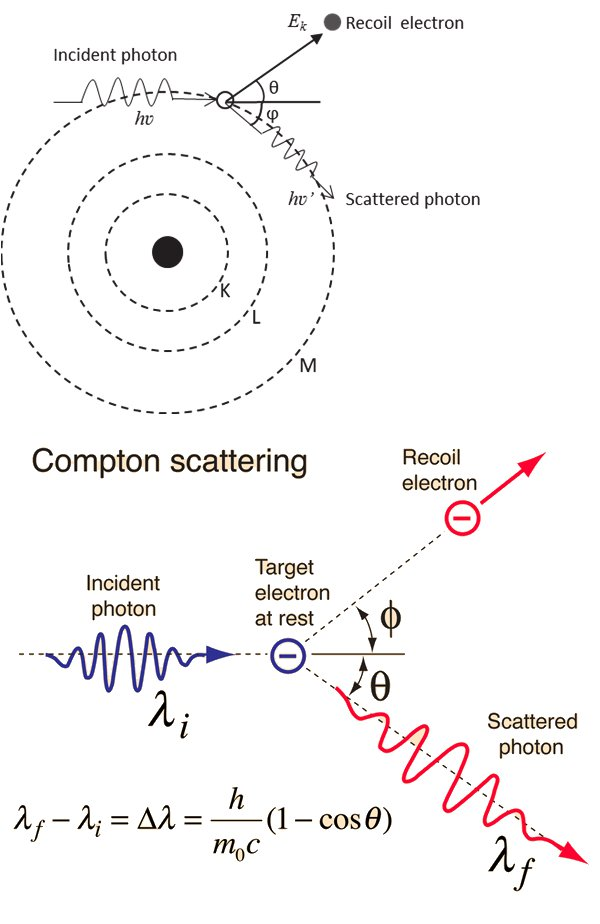
\includegraphics[width=0.8\columnwidth]{images/theory.png}
    \caption{An illustration depicting Compton scattering}
    \label{th:1}
\end{figure}

\subsection{Wave Particle Duality}

Light acts as both a wave and a particle, according to the wave-particle duality of light, and the Compton effect offered experimental proof that photons, which are light particles, have both wave-like and particle-like qualities. Using the conservation of momentum and energy in particle-photon collisions, we find that the wavelength of the scattered ray is greater than the wavelength of the incident ray, and that the observed shift in the wavelength of scattered photons is directly related to the energy and momentum exchanged between the photon and the electron.

Compton scattering is an example of inelastic collision and can be expressed in following way:

\begin{align*}\gamma + e \rightarrow \gamma^{'} + e^{'}\end{align*}

where $\gamma$ and $\gamma^{'}$  are the incident and scattered photons respectively, and e and $e^{'}$ are the initial and final electrons respectively.


The derivation of Compton scattering is based on two principles conservation of energy and conservation of momentum to the interaction between the photon and the electron. Let's assume that the photon has an initial energy of E and is incident on an electron at rest. After the interaction, the scattered photon has an energy of $E^{'}$ and moves in anew direction, while the electron recoils with a final momentum $p^{'}$. Using conservation of energy, we can write:

\begin{align}E + mc^2 = E^{'} \sqrt{m^2c^4+p^{'2}c^2}\end{align}

where m is the mass of the electron, and c is the speed of light. Using conservation of momentum, we can write:

\begin{align}p_{\gamma} = p^{'}_{\gamma} + p^{'}_{e}\end{align}

where $p_{\gamma}$ and $p^{'}_{\gamma}$ are the momenta of the incident and scattered photons, respectively, and $p^{'}_{e}$ is the momentum of the recoiling electron. The shift of the wavelength ($\Delta\lambda$) increased with scattering angle according to the Compton formula as more scattering angle implies greater loss in energy:

\begin{align}\Delta\lambda = \lambda_\theta - \lambda_0 = \frac{h}{m_ec}\left(1-\cos\theta\right)\end{align}

where $\lambda_\theta$ and $\lambda_0$ are wavelengths of scattered and initial photons respectively, $h$ is Planck's constant, $m_e$ is the rest mass of the electron, $c$ is the velocity of light, $\theta$ and $\phi$ are angles of scattered photon and recoil electron respectively. The value of ( $h/m_ec = 0.02426\,\angstrom$) is known as the Compton wavelength of the electron. 

% In this length scale, we can't talk about a single particle. We have to take into account of particle antiparticle pair that creates because of energy uncertainty.
In terms of energy, Eq. 3 can be rewritten as:

\begin{align}E_\theta = \frac{E_0}{(1+\gamma)(1-\cos\theta)}\end{align}

As a result, Compton scattering is significantly energy-dependent, and the relevant energy scale is determined by the ratio of input photon energy to electron rest energy. The fractional shift in energy is considerable if this ratio is big, and negligible if this ratio is small. Compton scattering is important only when the incoming photon energy is a considerable proportion of the electron's rest energy. The equation also demonstrates that the change in wave length of the scattered photon is proportional to the scattering angle and the photon's original energy. 
For high-energy photons ($\lambda << 0.02 \angstrom$ or $E >> 511$ keV), the wavelength of the scattered photon is comparable to the Compton wavelength, while for low-energy photons ($E << 511$ keV), the Compton shift is negligible. In the non-relativistic regime, Compton scattering closely aligns with the predictions of classical Thomson scattering.

It also illustrates that the scattered photon loses energy, and this lost energy is passed to the recoiling electron.

Using quantum mechanical calculations, Klein-Nishina correctly formulated the differential Compton scattering cross-section formula. This equation is written as follows:

\begin{equation}
    \begin{split}
        \frac{d\sigma}{d\Omega} = & r_o^2\left[\frac{1+ \cos^2\theta}{2(1+\gamma(1-\cos\theta)^2)}\right] \times \\
        & \left[1+\frac{\gamma^2(1-\cos\theta)^2}{(1+ \cos^2\theta)(1+\gamma(1-\cos\theta))}\right]
    \end{split}
    \label{eq:1}
\end{equation}

where, $r_o=\frac{e}{4\pi\epsilon_om_ec^2} = 2.8179 \times 10^{-15}$ m is the classical electron radius.

For dispersed photons, gamma rays from a Cs$^{137}$ source are used in this experiment. A calibrated scintillation detector set at varying scattering angles determines differences in incoming and scattered energy and wavelength of photons. By computing the calibration factor $C$ using the method below, the relative intensities $I_\theta$ of the scattered radiation peaks may be compared with the predictions of the Klein-Nishina formula for the differential effective cross-section $\frac{d\sigma}{d\Omega}$. Thus:

\begin{align} C=\frac{1}{n}\sum_{\theta=0}^{n}\frac{I_\theta}{\left(\frac{d\sigma}{d\Omega}\right)}\end{align}

	
% ======================================================================================
\section{Experimental Setup}

\subsection*{Apparatus}

\begin{enumerate}
    \item Cs-137 radioactive gamma source
    \item Mixed radioactive source for calibration (Am-241 and Cs-137)
    \item Lead block source holder with a 12 mm diameter hole at the center to accommodate radioactive sources, and an additional blind hole for inserting a steel pin as an angular direction indicator
    \item NaI scintillation detector with a holder and lead shielding to define the direction of incoming gamma radiation
    \item High voltage power supply (1.5 kV)
    \item Cylindrical pure aluminum or copper rod to be used as a scattering body
    \item Movable lead shielding to reduce the intensity of unscattered gamma radiation
    \item Multichannel analyzer (256 channels) with associated software ( CASSY Lab 2) installed on a desktop PC.
    \item Experimental panel with a graduated angular scale\\
\end{enumerate}

A radioactive Cs-137 source emits
662 keV gamma rays, which escape through a small
opening in the shielded cavity (Fig. \ref{th:2}). The collimated beam
is directed onto an aluminum rod, serving as the
target or scatterer.
Electrons in the target scatter a portion of the gamma rays, which are then
detected and counted by the scintillation detector.

A scintillation detector is a device used to detect and
measure ionizing radiation. It operates by utilizing
the excitation effect of incoming radiation on a scintillating material, which produces light pulses that
are subsequently detected by photodetectors such as a photomultiplier
tube (PMT), a charge-coupled device (CCD) camera.

The resulting signal is processed by a multichannel
analyzer (MCA), and the corresponding spectrum is
displayed on the computer. By adjusting the source
to various angles on the angular scale of the experimental panel, the scattered radiation is measured to analyze the angular dependence of Compton scattering.

\begin{figure}
    \centering
    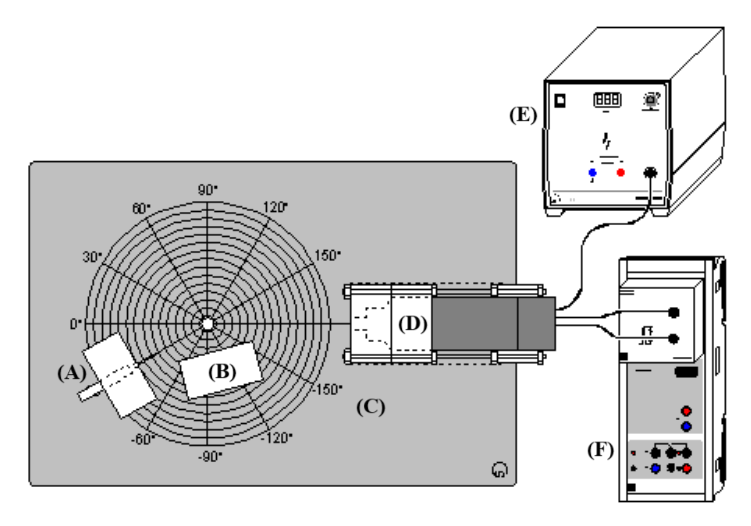
\includegraphics[width=1\columnwidth]{images/setup.png}
    \caption{The experimental setup, with components (A) the Lead block source holder (B) Additional Lead block for shielding (C) graduated angular scale (D) the scintillation detector (E) High-voltage power supply and (F) MCA connected to a computer}
    \label{th:2}
\end{figure}